\documentclass[a4paper,12pt]{article}
\usepackage{ amssymb }
\usepackage{mathtools}
\usepackage{listings}
\usepackage{color}
\usepackage[utf8]{inputenc}
\usepackage{amsmath}
\usepackage{tikz}
\DeclarePairedDelimiter\ceil{\lceil}{\rceil}
\DeclarePairedDelimiter\floor{\lfloor}{\rfloor}

\definecolor{codegreen}{rgb}{0,0.6,0}
\definecolor{codegray}{rgb}{0.5,0.5,0.5}
\definecolor{codepurple}{rgb}{0.58,0,0.82}
\definecolor{backcolour}{rgb}{0.95,0.95,0.92}
\definecolor{highlightcolor}{rgb}{0.8, 0.9, 0.9}

\lstdefinestyle{mystyle}{
    backgroundcolor=\color{backcolour},   
    commentstyle=\color{codegreen},
    keywordstyle=\color{magenta},
    numberstyle=\tiny\color{codegray},
    stringstyle=\color{codepurple},
    basicstyle=\footnotesize,
    breakatwhitespace=false,         
    breaklines=true,                 
    captionpos=b,                    
    keepspaces=true,                 
    numbers=left,                    
    numbersep=5pt,                  
    showspaces=false,                
    showstringspaces=false,
    showtabs=false,                  
    tabsize=2
}
 
\lstset{style=mystyle}

\newcommand*\Suppressnumber{%
  \lst@AddToHook{OnNewLine}{%
    \let\thelstnumber\relax%
     \advance\c@lstnumber-\@ne\relax%
    }%
}

\begin{document}

\noindent{
\framebox {
\begin{minipage}{\dimexpr\textwidth-2\fboxsep-2\fboxrule\relax}
\vspace{2mm}
1. \textbf{Comparison of running times}: For each function $f(n)$ and time $t$ in the 
following table, determine the largest size $n$ of a problem that can be solved
in time $t$, assuming that the algorithm to solve the problem takes $f(n)$ microseconds. 

\vspace{4mm}

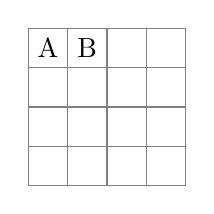
\begin{tikzpicture}
\draw[step=0.5cm,color=gray] (-1,-1) grid (1,1);
\node at (-0.75,+0.75) {A};
\node at (-0.25,+0.75) {B};

\end{tikzpicture}

1 second, 1 minute, 1 hour, 1 day, 1 month, 1 year, 1 century.

$\lg n$, $\sqrt n$, $n$, $n \lg n$, $n^2$, $n^3$, $2^n$, $n!$
\vspace{2mm}
\end{minipage}
}
}

For $f(n) = \lg n$. 1 second = $10^6$ microseconds.

If we can solve a problem of size $n$, and the operation 
takes $f(n) = \lg n$, ten 1 second is $\lg n = 10^6$.

$f(n) = \lg n$

n = 2 will be 1 microsecond.

n = 4 will be 2 microseconds.

n = 8 will be 3 microseconds.

n = 256 will be 8 microseconds.

n = 65,536 will be 16 microseconds.

n = 16,777,216 will be 24 microseconds.

Since 1 second has $10^6$ microseconds, we can solve a problem of size $n = 2^{10^6}$ in 1 second.

$f(n) = \lg n$

1 second is $n = 2^{10^6}$.

1 minute is $n =2^{6 \times 10^7}  $.

1 hour is $n = 2^{3.6 \times 10^9}$.

1 day is $n = 2^{8.64 \times 10^{10}}$

1 month is $n = 2^{2.59 \times 10^{12}}$

1 year is $n = 2^{3.11 \times 10^{13}}$

1 century  is $n = 2^{3.11 \times 10^{15}}$

===

$f(n) = \sqrt n$

1 second is $n = 10^{12}$.

1 minute is $n = (60 \times 10^6)^2 = (6 \times 10^7)^2 = (36 \times 10^{14}) = 3.6 \times 10^{15}$.

1 hour is $n = (60 \times 6 \times 10^7)^2 = (3.6 \times 10^9)^2 = 12.96 \times 10^{18} = 1.296 \times 10^{19}$

1 day is $n = (24 \times 3.6 \times 10^{9})^2 = (8.64 \times 10^{10})^2 = 74.6496 \time 10^{20}  = 7.465 \times 10^{21}$

1 month is $n = (30 \times 8.64 \times 10^{10})^2 = (259.2 \times 10^{10})^2 = (2.592 \times 10^{12})^2 = 6.7185 \times 10^{24}$

1 year is $n = (12 * 2.592 \times 10^{12})^2 = (31.104 \times 10^{12})^2 = (3.11 \times 10^{13})^2 = 9.672 \times 10^{26}$.

Working.

\noindent{
\framebox {
\begin{minipage}{\dimexpr\textwidth-2\fboxsep-2\fboxrule\relax}
\vspace{2mm}
2. \textbf{Insertion sort on small arrays in merge sort}: 
Although merge sort runs in $\Theta(n\lg n)$ worst-case
 time and insertion sort runs in $\Theta(n^2)$ worst-case 
 time, the constant factors in insertion sort make it 
 faster for small $n$. Thus, it makes sense to use insertion 
 sort within merge sort when subproblems become sufficiently
 small. Consider a modification to merge sort in which 
 $n/k$ sublists of length $k$ are sorted using insertion sort, 
 and then merged using the standard merging mechanism, 
 where $k$ is a value to be determined.
 
 \vspace{2mm}
 a. Show that the $n/k$ sublists, each of length $k$, can be
 sorted by insertion sort in $\Theta(nk)$ worst-case time.
 
  \vspace{2mm}
 b. Show that the sublists can be merged in $\Theta(n \lg (n/k)$
 worst-case time.
 
  \vspace{2mm}
 c. Given that the modified algorithm runs in $\Theta(nk + n\lg (n/k)$
 worst-case time, what is the largest asymptotic ($\Theta$-notation)
 value of $k$ as a function of $n$ for which the modified algorithm has
 the same asymptotic running time as standard merge sort?
 
  \vspace{2mm}
 d. How should $k$ be chosen in practice?
\vspace{2mm}
\end{minipage}
}
}

Working.

\noindent{
\framebox {
\begin{minipage}{\dimexpr\textwidth-2\fboxsep-2\fboxrule\relax}
\vspace{2mm}
3. \textbf{Inversions}: Let $A[1..n]$ be an array of $n$ distinct numbers. If $i < j$ 
and $A[i] > A[j]$ then the pair $(i.j)$ is called an \textbf{inversion}
of $A$.

\vspace{2mm}
a. List the five inversions of the array $(2, 3, 8, 6, 1)$.

\vspace{2mm}
b. What array with elements from the set $\{1, 2, ..., n\}$ has the 
most inversions? How many does it have?

\vspace{2mm}
c. What is the relationship between the running time of insertion 
sort and the number of inversions? Justify your answer.

\vspace{2mm}
d. Give an algorithm that determines the number of inversions
in any permutation on $n$ elements in $\Theta(n \lg n)$ wore-case times. 
(Hint: Modify merge sort).
\vspace{2mm}
\end{minipage}
}
}

The five inversions of $A = (2, 3, 8, 6, 1)$ are $(2, 1)$, $(3,1)$, $(8,6)$, $(8,1)$ and $(6,1)$.

Working.



\end{document}
